\section{More Simulation Results}\label{appendix:more_result}

\paragraph{Pairwise Distance Estimation}
In Figure \ref{fig:gaussian}, \ref{fig:sparse}, \ref{fig:very_sparse}, we compare the performance of Gaussian, Sparse, Very Sparse random maps on the pairwise distance estimation problem with $d = 2500, 10000, 40000, N= 2$. Additionally, we compare their performance for $d = 125000, N = 3$ in Figure \ref{fig:triple_krao}.

\begin{figure}[ht!]
	\centering
	\begin{subfigure}{0.32\textwidth}
		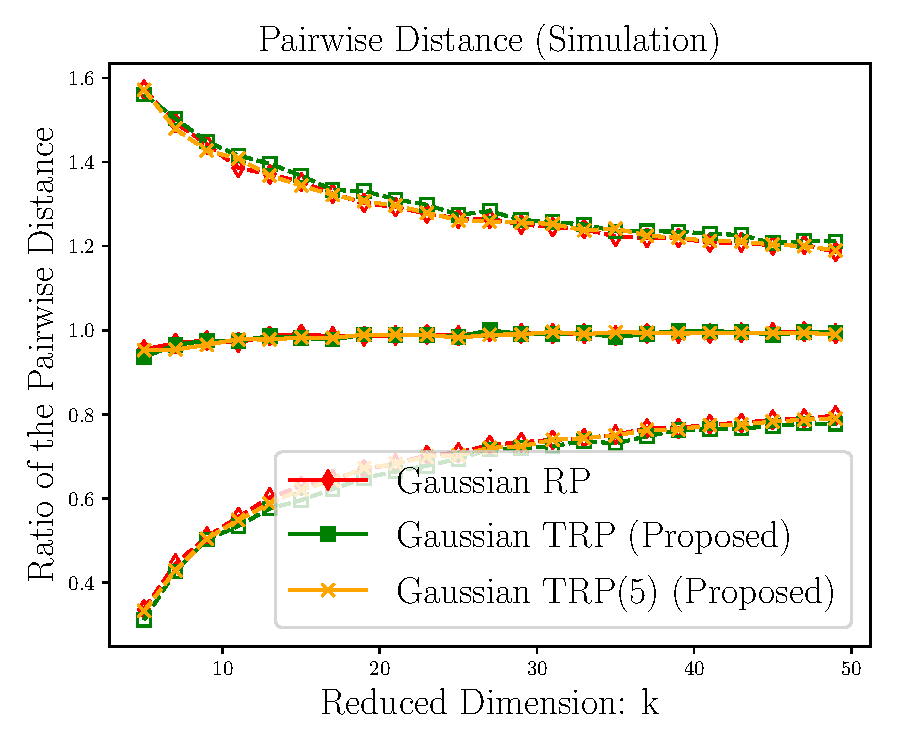
\includegraphics[scale = 0.3]{figure/dist_g_d2500.pdf}
	\end{subfigure}
	\begin{subfigure}{0.32\textwidth}
		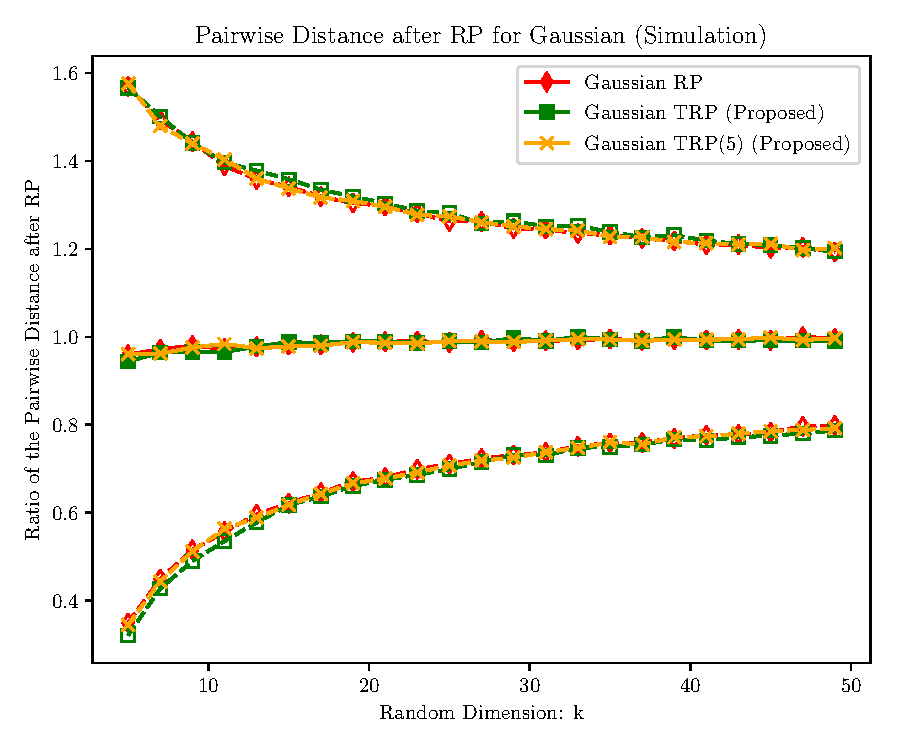
\includegraphics[scale = 0.3]{figure/dist_g_d10000.pdf}
	\end{subfigure}
	\begin{subfigure}{0.32\textwidth}
		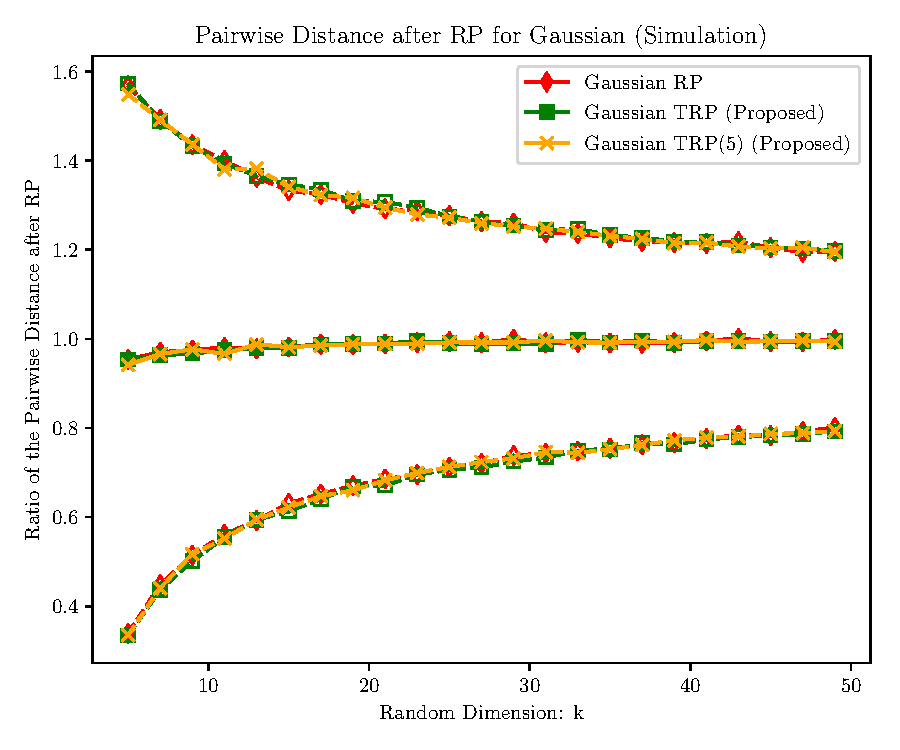
\includegraphics[scale = 0.3]{figure/dist_g_d40000.pdf}
	\end{subfigure}
	\\
	\caption{Average ratio of the pairwise distance for simulation data using Gaussian RP: \textit{The  plots correspond to the simulation for Gaussian RP, TRP, $\textup{TRP}_5$ respectively with $n = 20, d = 2500, 10000, 40000$ and each data vector comes from $N(\mathbf{0}, \mathbf{I})$. The dashed line represents the error bar 2 standard deviation away from the average ratio.}} 
	\label{fig:gaussian}
\end{figure}

\begin{figure*}[ht!]
	\centering
	\begin{subfigure}{0.32\textwidth}
		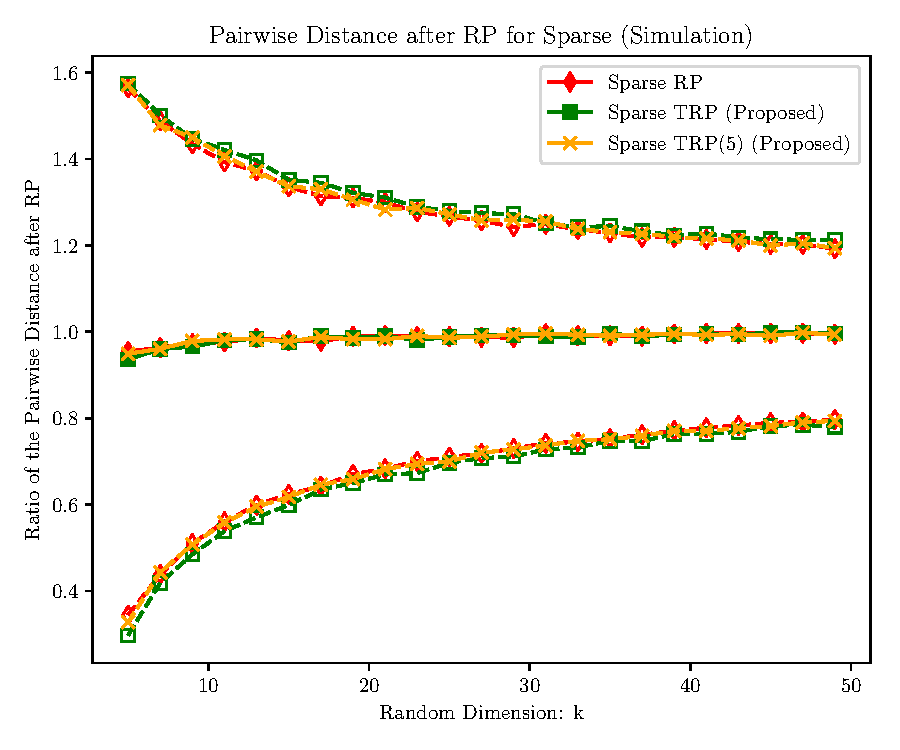
\includegraphics[scale = 0.3]{figure/dist_sp0_d2500.pdf}
	\end{subfigure}
	\begin{subfigure}{0.32\textwidth}
		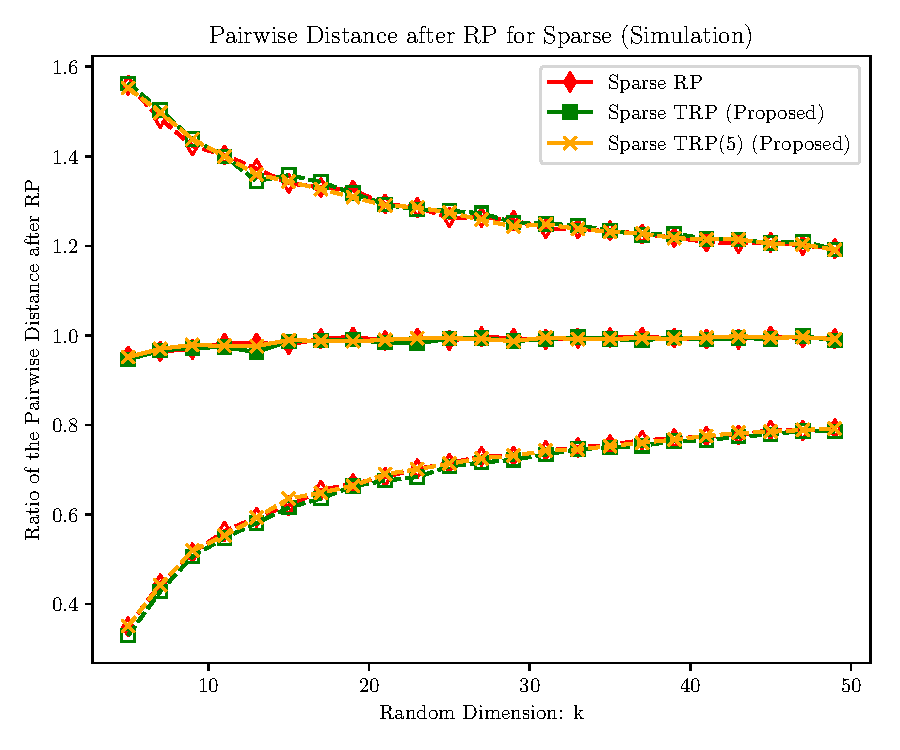
\includegraphics[scale = 0.3]{figure/dist_sp0_d10000.pdf}
	\end{subfigure}
	\begin{subfigure}{0.32\textwidth}
		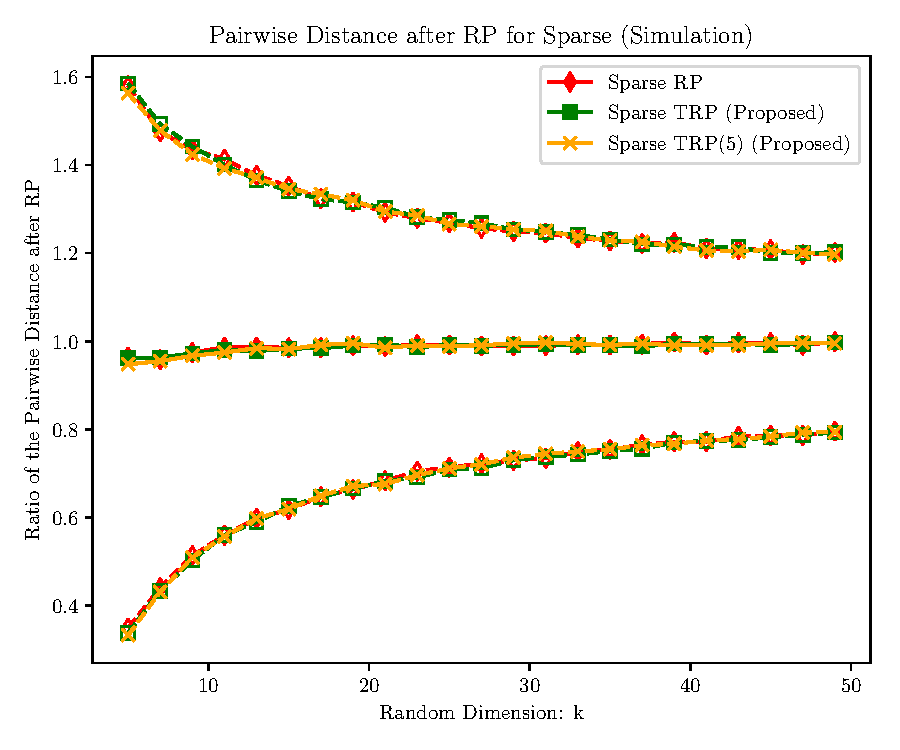
\includegraphics[scale = 0.3]{figure/dist_sp0_d40000.pdf}
	\end{subfigure}\\
	\caption{Average ratio of the pairwise distance for simulation data using Sparse RP: \textit{The  plots correspond to the simulation for Sparse RP, TRP, $\textup{TRP}_5$ respectively with $n = 20, d = 2500, 10000, 40000$ and each data vector comes from $N(\mathbf{0}, \mathbf{I})$. The dashed line represents the error bar 2 standard deviation away from the average ratio.}} 
	\label{fig:sparse}
\end{figure*}

\begin{figure*}[ht!] 
	\centering
	\begin{subfigure}{0.32\textwidth}
		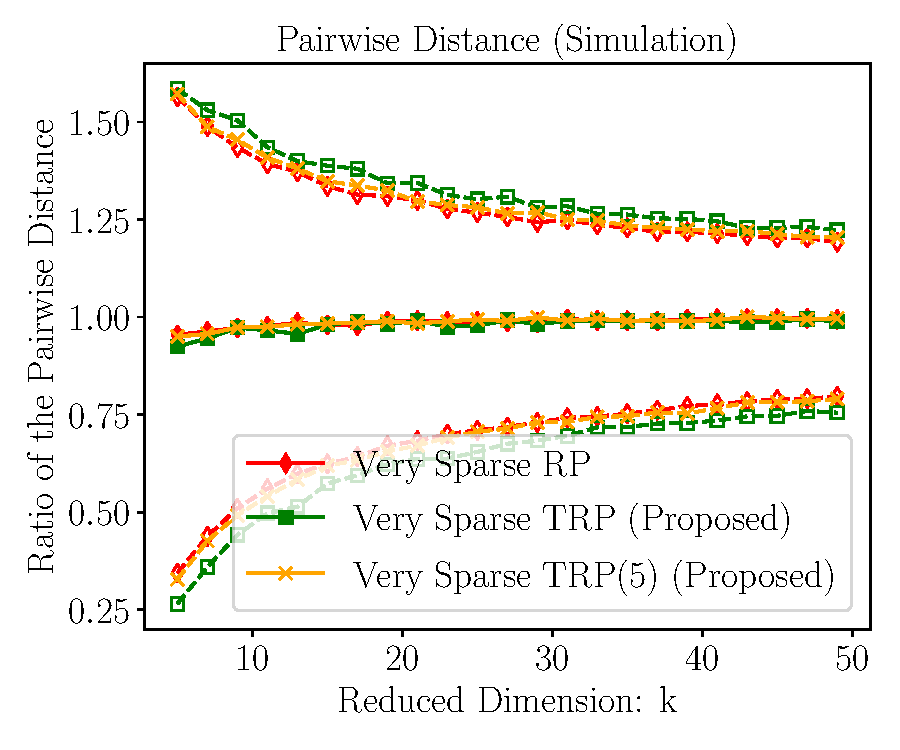
\includegraphics[scale = 0.3]{figure/dist_sp1_d2500.pdf}
	\end{subfigure}
	\begin{subfigure}{0.32\textwidth}
		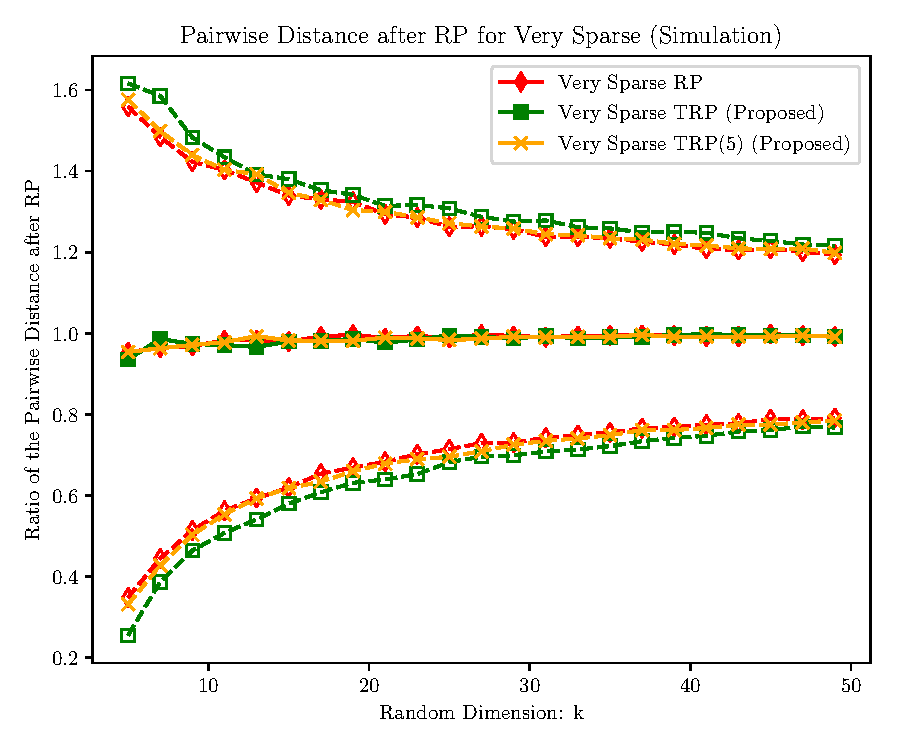
\includegraphics[scale = 0.3]{figure/dist_sp1_d10000.pdf}
	\end{subfigure}
	\begin{subfigure}{0.32\textwidth}
		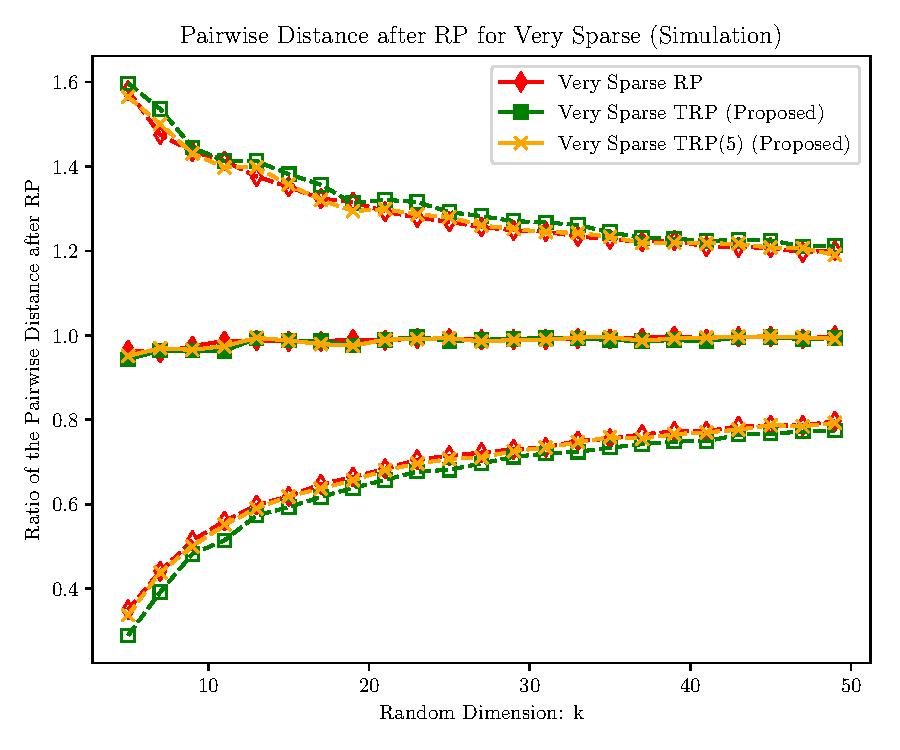
\includegraphics[scale = 0.3]{figure/dist_sp1_d40000.pdf}
	\end{subfigure}\\
	\caption{Average ratio of the pairwise distance for simulation data using Very Sparse RP: \textit{The plots correspond to the simulation for Very Sparse RP, TRP, $\textup{TRP}_5$ respectively with $n = 20, d = 2500, 10000, 40000$ and each data vector comes from $N(\mathbf{0}, \mathbf{I})$. The dashed line represents the error bar 2 standard deviation away from the average ratio.}} 
	\label{fig:very_sparse}
\end{figure*}

\begin{figure*}[ht!] 
	\centering
	\begin{subfigure}{0.32\textwidth}
		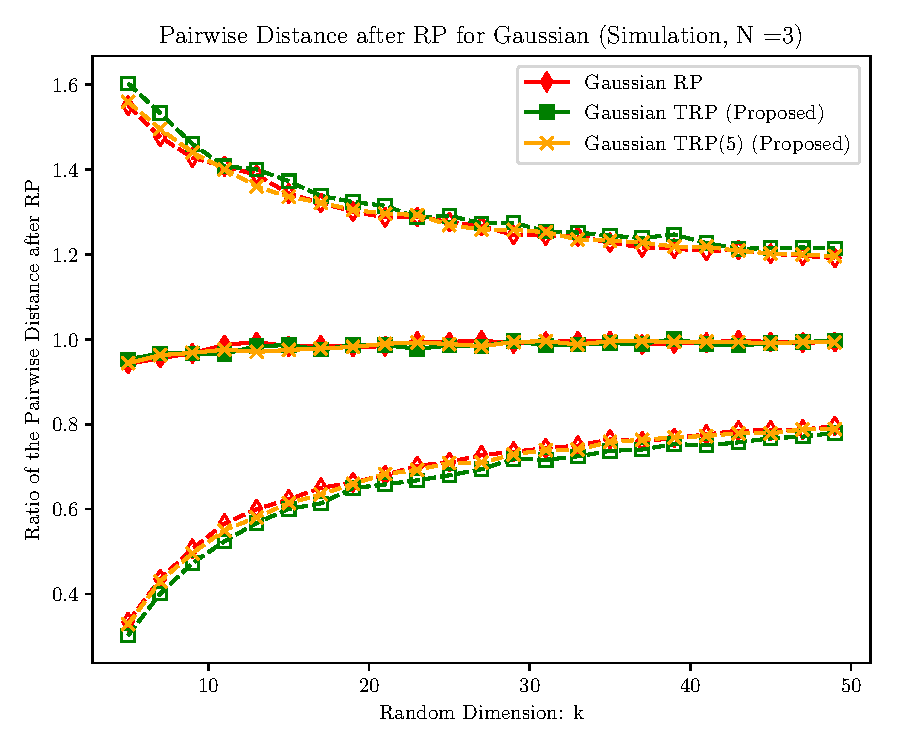
\includegraphics[scale = 0.3]{figure/dist_g_d125000.pdf}
	\end{subfigure}
	\begin{subfigure}{0.32\textwidth}
		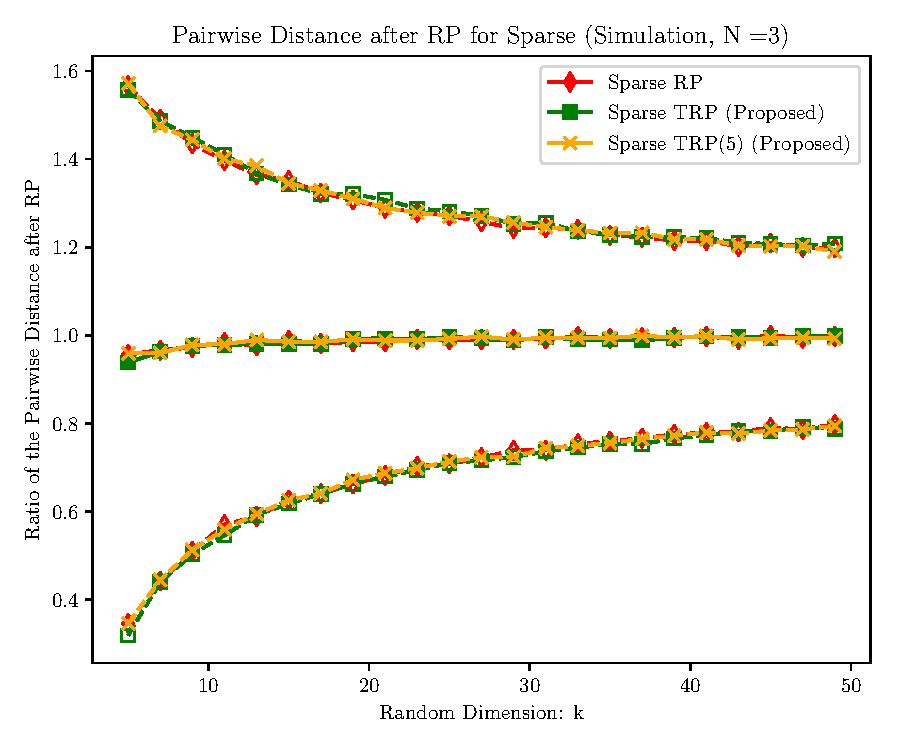
\includegraphics[scale = 0.3]{figure/dist_sp0_d125000.pdf}
	\end{subfigure}
	\begin{subfigure}{0.32\textwidth}
		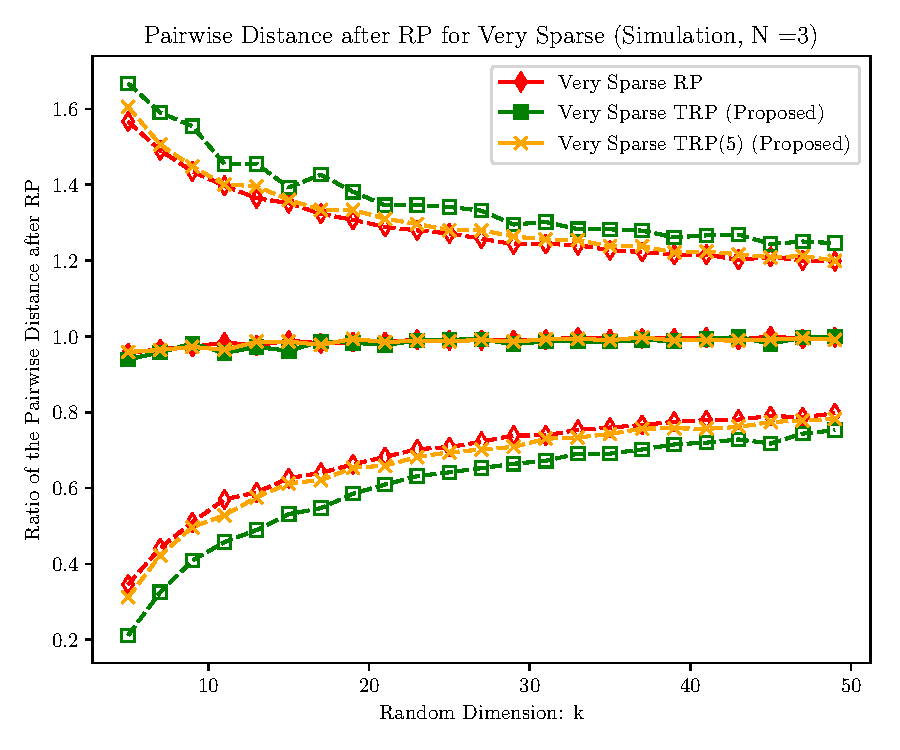
\includegraphics[scale = 0.3]{figure/dist_sp1_d125000.pdf}
	\end{subfigure}\\
	\caption{Average ratio of the pairwise distance for simulation data using: \textit{The plots correspond to the simulation for Gaussian, Sparase, Very Sparse RP, TRP, $\textup{TRP}_5$ respectively with $n = 20, d = d_1d_2d_3 = 50 \times 50 \times 50 = 125000$ and each data vector comes from $N(\mathbf{0}, \mathbf{I})$. The dashed line represents the error bar 2 standard deviation away from the average ratio.}} 
	\label{fig:triple_krao}
\end{figure*}


\paragraph{Pairwise Cosine Similarity Estimation} 
The second experiment is to estimate the pairwise cosine similarity, i.e. $\frac{\mathbf{x}_i \cdot \mathbf{x}_j}{\|\mathbf{x}_i\|_2 \|\mathbf{x}_j\|_2}$ for $\mathbf{ x}_i, \mathbf{x}_j$. We use both the simulation data ($d = 10000$) and the MNIST data ($d = 784, n = 60000$). We experiment with Gaussian, Sparse, Very Sparse RP, TRP, and $\textup{TRP}_5$ with the same setting as above ($k = 50$). We evaluate the performance by the average root mean square error (RMSE). The results is given in Table  \ref{tbl:mnist_inner_prod}, \ref{tbl:sim_inner_prod}.  

\begin{table}[ht!]
\centering
\begin{tabular}{l|l|l|l}
       & Gaussian        & Sparse          & Very Sparse     \\ \hline
RP     & 0.1409 (0.0015) & 0.1407 (0.0013) & 0.1412 (0.0014) \\ \hline
TRP    & 0.1431 (0.0016) & 0.1431 (0.0015) & 0.1520 (0.0033) \\ \hline
$\textup{TRP}_5$ & 0.1412 (0.0012) & 0.1411 (0.0015) & 0.1427 (0.0014)
\end{tabular}
\caption{RMSE for the estimate of the pairwise inner product of the simulation data ($d = 10000, k = 50, n = 100 $), where standard error is in the parentheses.
}\label{tbl:sim_inner_prod}
\end{table}
